
Boundary conditions of this exercise
\begin{itemize}
\item two-dimensional
\item Cartesian domain
\item Continuous Galerkin method
\item most of commonly used elements 
\item Dirichlet boundary conditions
\item isoparametric mapping
\end{itemize}



is there still a need for dNNNN and dNNN ?


The idea here is to create a library of basis functions and quadrature rules, as well as 
other FE-related tools so as to be able to write much more compact FE codes. 

There are three files which contain all the required tools to build most of a FE code:

\begin{itemize}

\item {\pythonfile FEbasis2D.py} contains 
\begin{lstlisting}
NNN(r,s,space):
dNNNdr(r,s,space):
dNNNds(r,s,space):
NNN_r(space):
NNN_s(space):
NNN_m(space):
visualise_nodes(space):
\end{lstlisting}



\item {\pythonfile FEtools.py} contains

\begin{lstlisting}
cartesian_mesh(Lx,Ly,nelx,nely,element):
export_mesh_to_ascii(x,y,filename):
export_connectivity_array_to_ascii(x,y,icon,filename):
export_mesh_to_vtu(x,y,icon,space,filename):
export_swarm_to_vtu(x,y,filename):
bc_setup(x,y,Lx,Ly,ndof,left,right,bottom,top):
J(m,dNdr,dNds,x,y):
assemble_K(K_el,A_sparse,iconV,mV,ndofV,iel):
assemble_G(G_el,A_sparse,iconV,iconP,NfemV,mV,mP,ndofV,ndofP,iel):
apply_bc(K_el,G_el,f_el,h_el,bc_val,bc_fix,iconV,mV,ndofV,iel):
\end{lstlisting}

\item {\pythonfile FEquadrature.py} contains

\begin{lstlisting}
quadrature(space,nqperdim):
qcoords_1D(nqperdim):
qweights_1D(nqperdim):
visualise_quadrature_points(space,nqpts):
\end{lstlisting}

\end{itemize}

\newpage
%--------------------------------------------------------------------
\section*{Supported element spaces}

\begin{center}
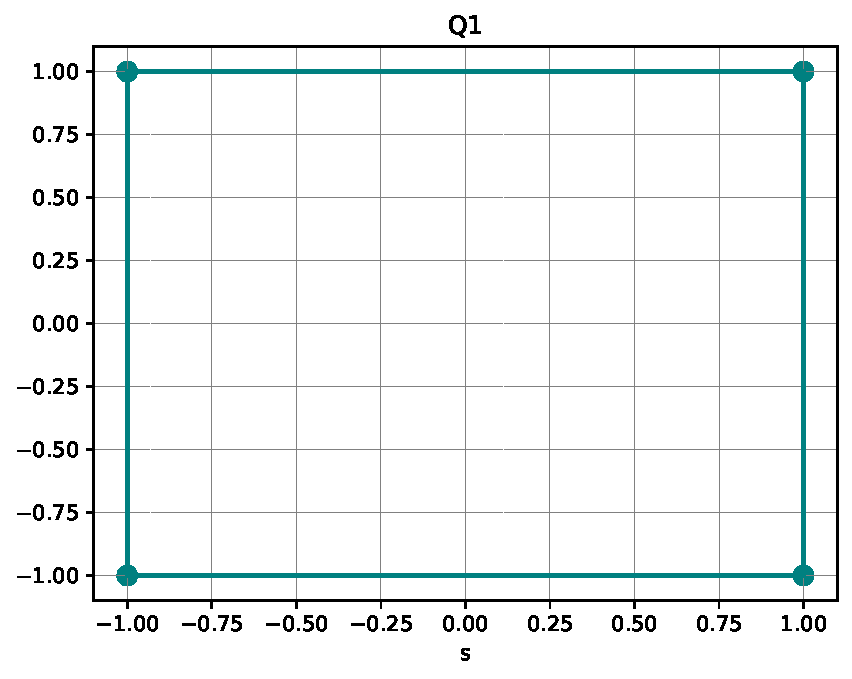
\includegraphics[width=4.5cm]{python_codes/fieldstone_120/spaces/Q1_nodes}
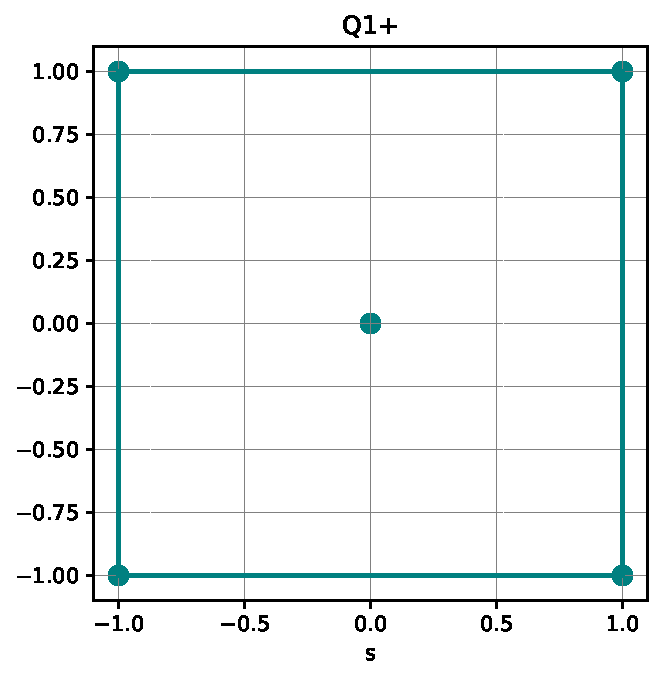
\includegraphics[width=4.5cm]{python_codes/fieldstone_120/spaces/Q1+_nodes}
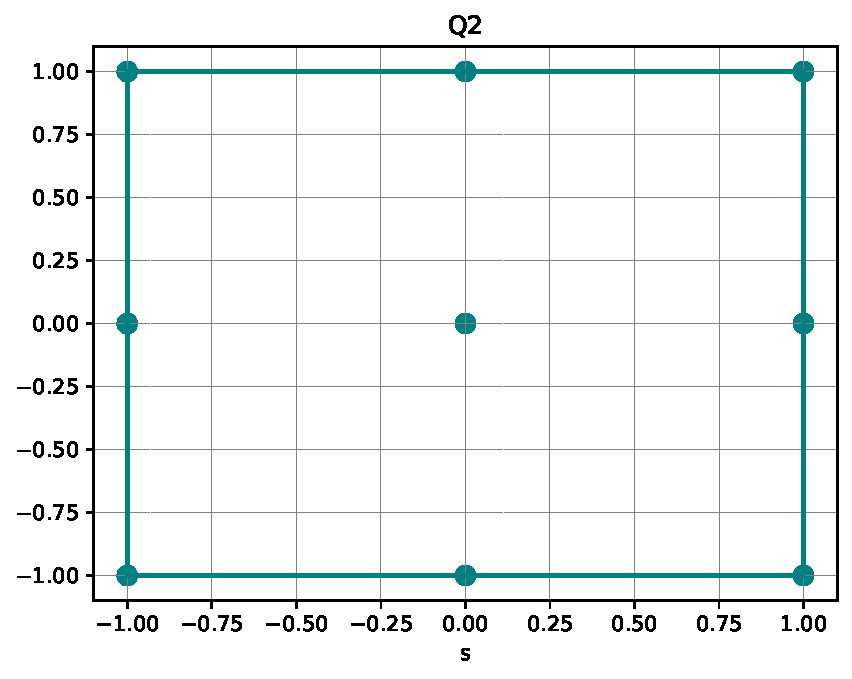
\includegraphics[width=4.5cm]{python_codes/fieldstone_120/spaces/Q2_nodes}\\
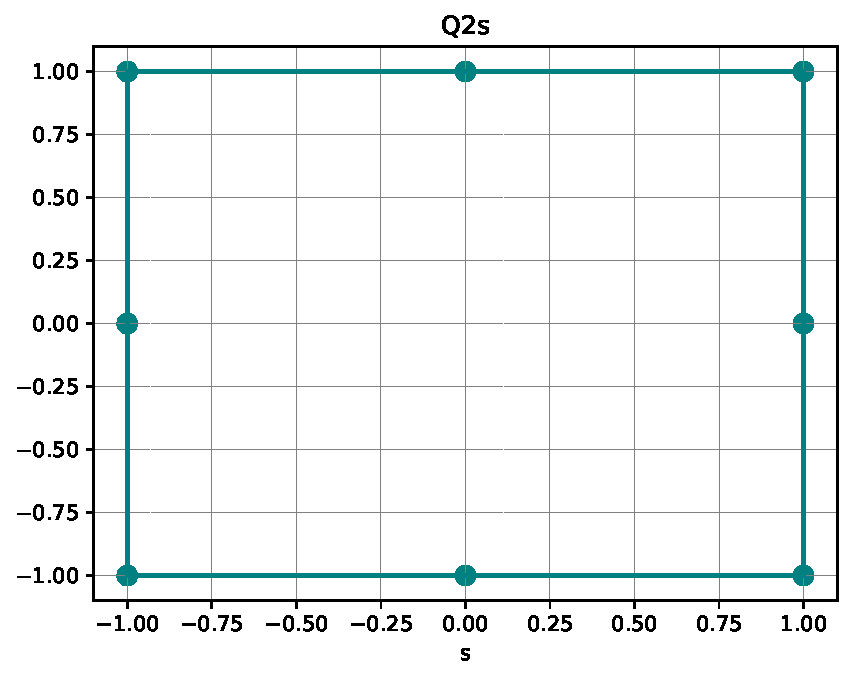
\includegraphics[width=4.5cm]{python_codes/fieldstone_120/spaces/Q2s_nodes}
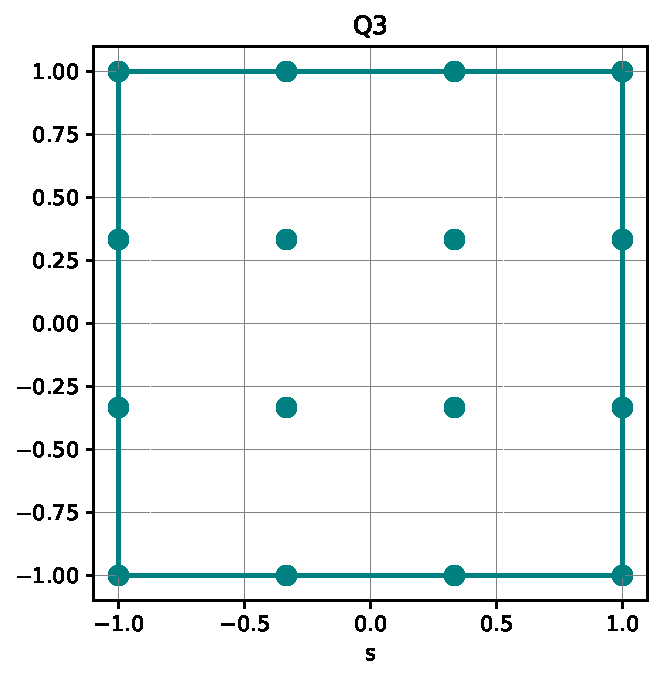
\includegraphics[width=4.5cm]{python_codes/fieldstone_120/spaces/Q3_nodes}
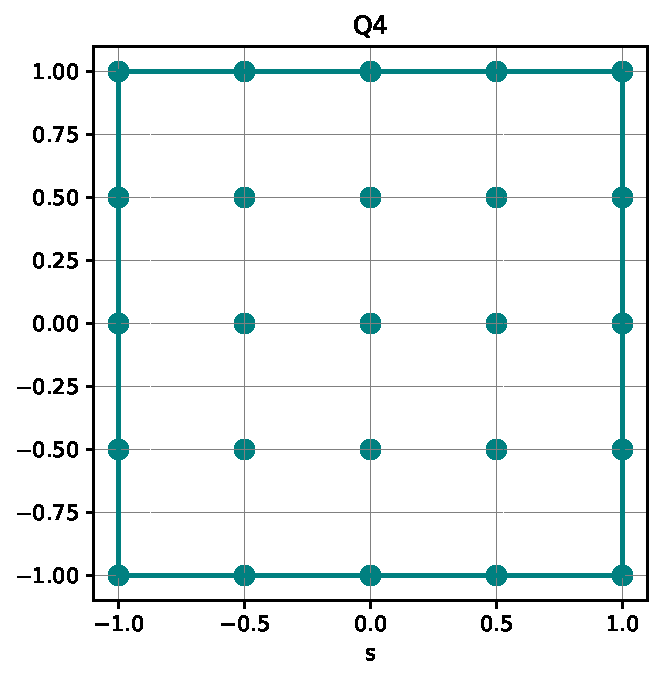
\includegraphics[width=4.5cm]{python_codes/fieldstone_120/spaces/Q4_nodes}\\
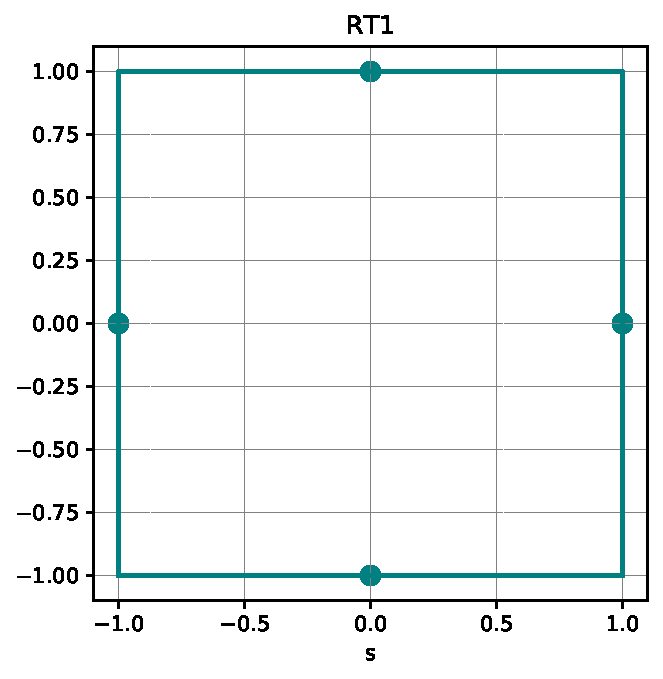
\includegraphics[width=3.3cm]{python_codes/fieldstone_120/spaces/RT1_nodes}
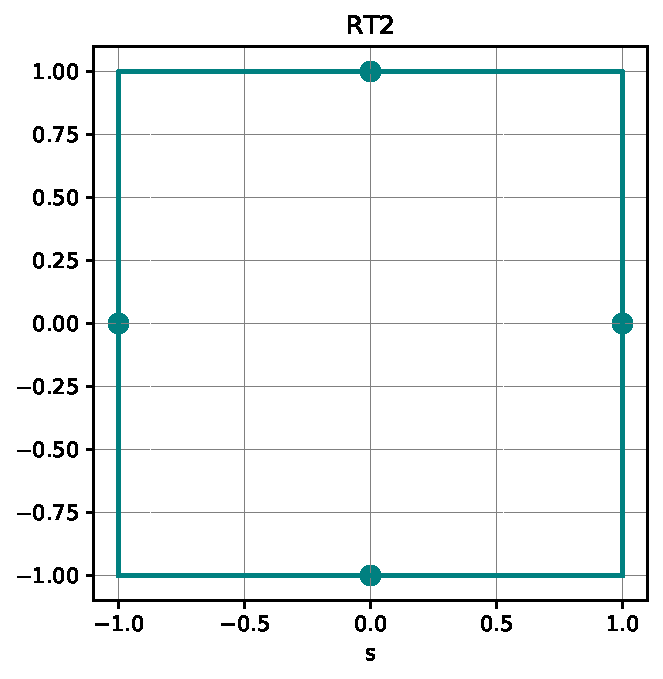
\includegraphics[width=3.3cm]{python_codes/fieldstone_120/spaces/RT2_nodes}
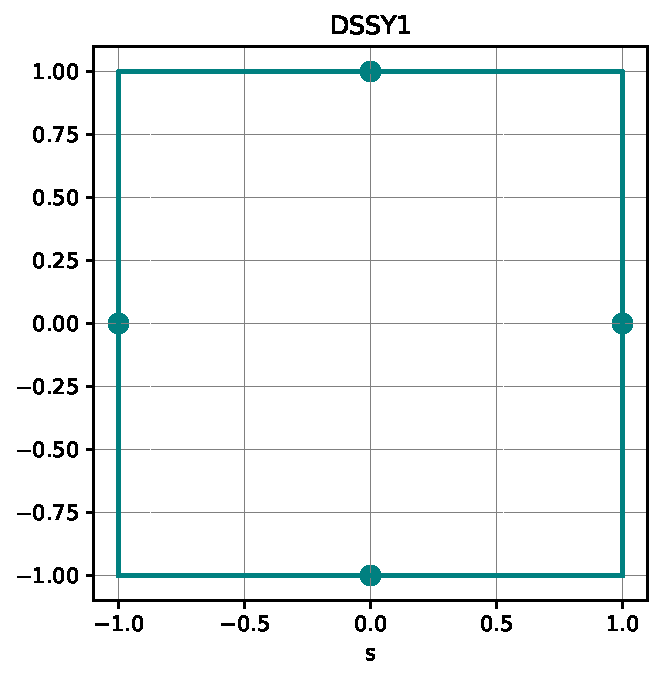
\includegraphics[width=3.3cm]{python_codes/fieldstone_120/spaces/DSSY1_nodes}
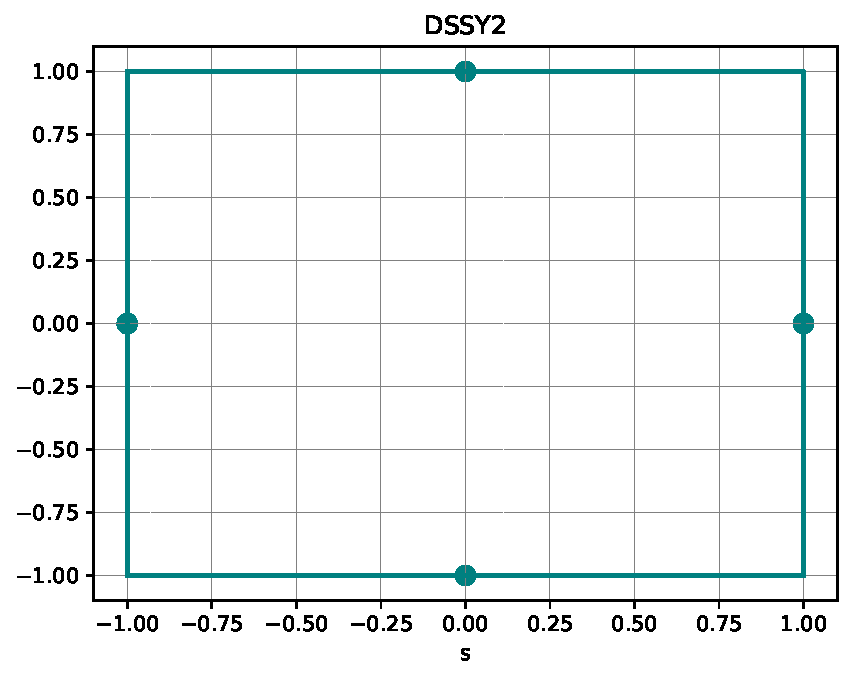
\includegraphics[width=3.3cm]{python_codes/fieldstone_120/spaces/DSSY2_nodes}\\
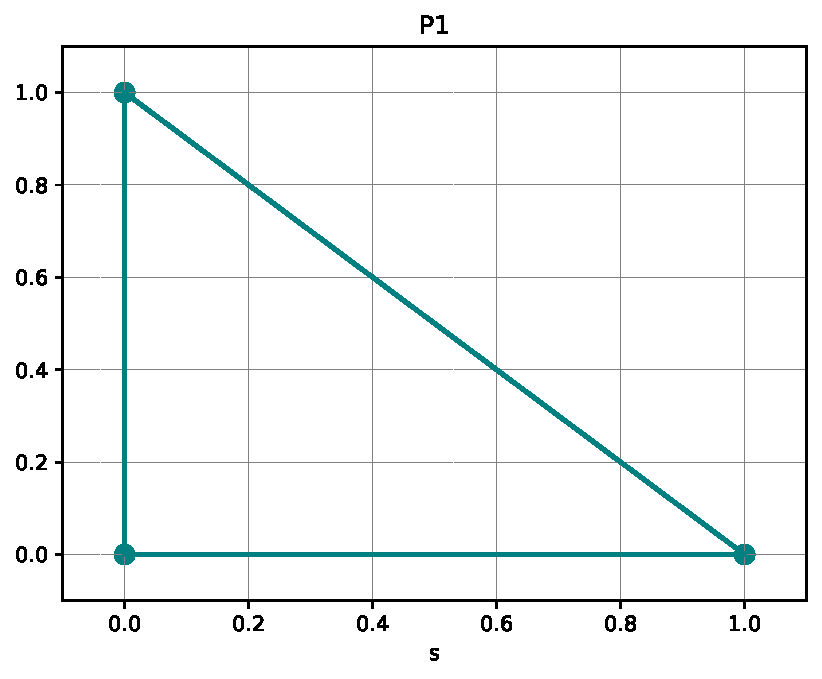
\includegraphics[width=4.cm]{python_codes/fieldstone_120/spaces/P1_nodes}
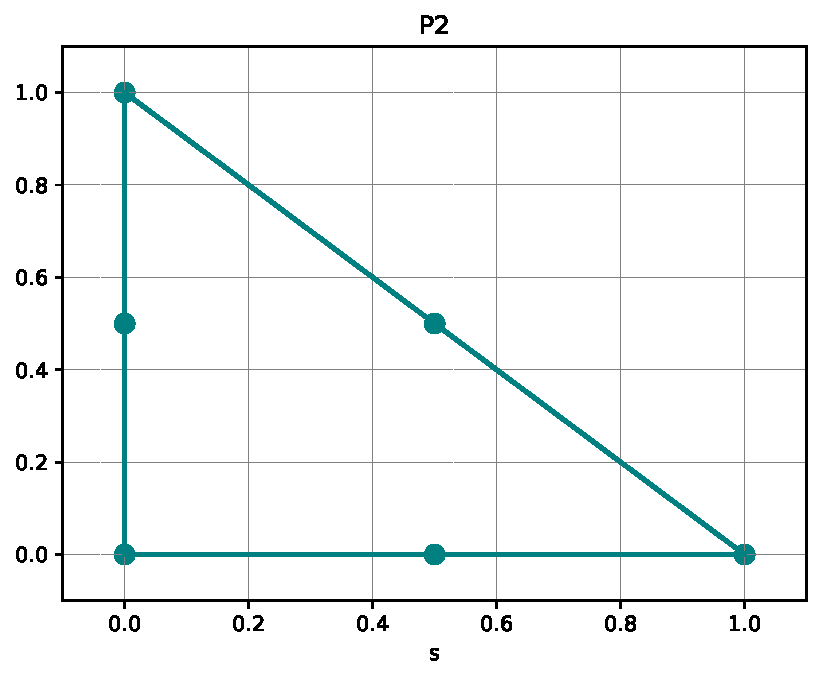
\includegraphics[width=4.5cm]{python_codes/fieldstone_120/spaces/P2_nodes}
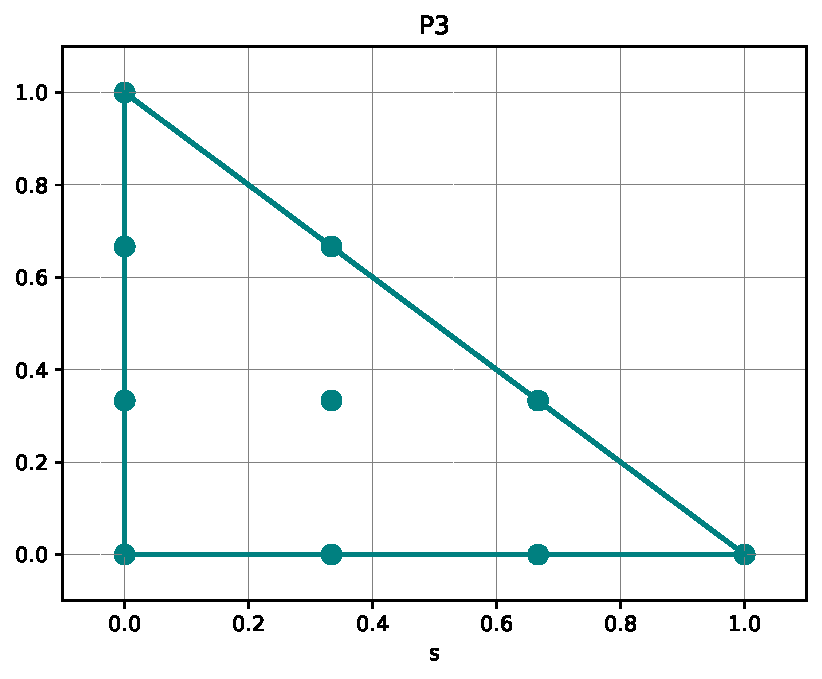
\includegraphics[width=4.5cm]{python_codes/fieldstone_120/spaces/P3_nodes}\\
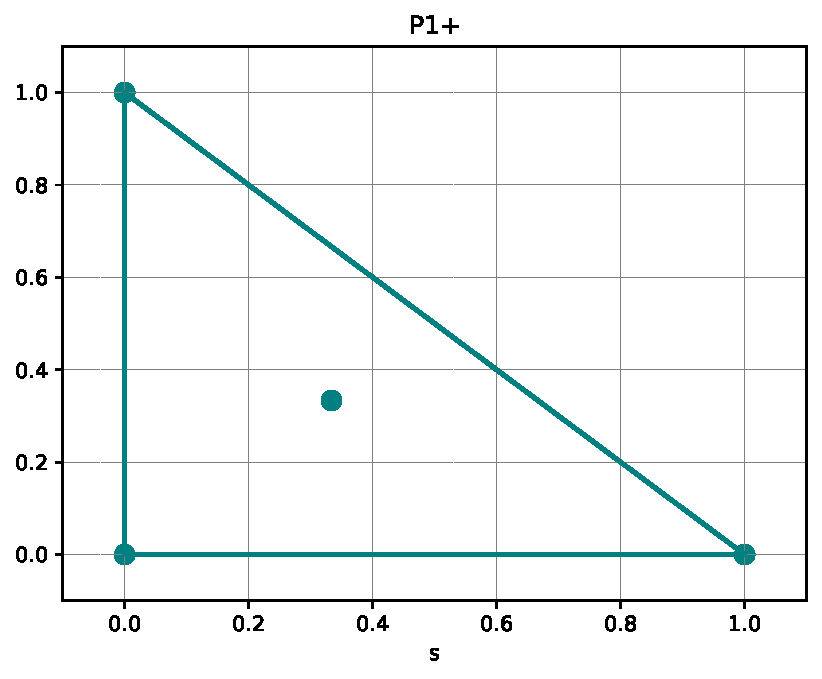
\includegraphics[width=4.5cm]{python_codes/fieldstone_120/spaces/P1+_nodes}
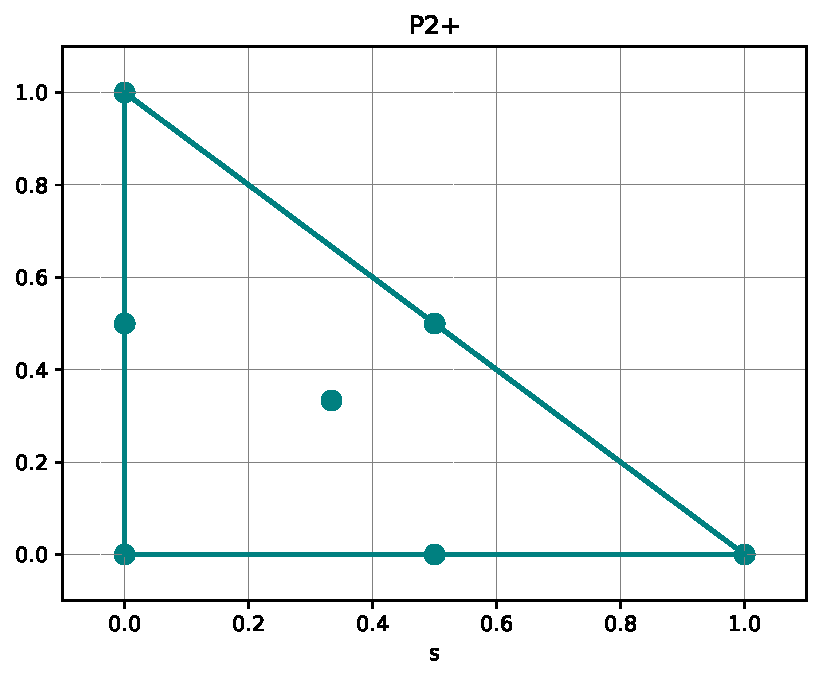
\includegraphics[width=4.5cm]{python_codes/fieldstone_120/spaces/P2+_nodes}
\end{center}

mesher: Q0,Q1,Q2,Q3,Q4, P0,P1,P2   missing P1+, P2+

\begin{tabular}{ccccccccccccc}
      & Q1P0 & Q1Q1 & Q2Q1 & Q3Q2 & Q4Q3 & Q1+Q1 & P1P0 & P2P1 & P3P2 & P2+P1 & P1+P1 \\
\hline
areas  & ok & & ok & ok &&&&&& \\ 
D\&H   &  \\
errors &  \\
vrms   &  \\
\hline
\end{tabular}


%-----------------------------------------------------------------------------
\section*{Finite element pairs for the Stokes equation}

\begin{itemize}
\item $Q_1\times Q_0$: see Section~\ref{ss:pairq1p0}
\item $Q_2\times Q_1$: see Section~\ref{ss:pairq2q1}
\item $Q_2\times P_{-1}$: see Section~\ref{ss:pairq2pm1}
\item $Q_3\times Q_2$: see Section~\ref{XXX}
\item $Q_4\times Q_3$: see Section~\ref{YYY}
\item $Q_1^+\times Q_1$: Quadrilateral mini, see Section~\ref{ss:}
\item $Q_2^{(8)}\times Q_1$: Serendipity, see Section~\ref{ss:}
\item $Q_1\times Q_0$-DSSY1: see Section~\ref{ss:}
\item $Q_1\times Q_0$-DSSY2: see Section~\ref{ss:}
\item $Q_1\times Q_0$-RT1: see Section~\ref{ss:RTq1p0}
\item $Q_1\times Q_0$-RT2: see Section~\ref{ss:RTq1p0}
\item $P_1\times P_0$: see Section~\ref{ss:}
\item $P_2\times P_1$: see Section~\ref{ss:p2p1}
\item $P_3\times P_2$: see Section~\ref{ss:}
\item $P_1^{+}\times P_{1}$: MINI, see Section~\ref{pair:mini}
\item $P_2^+\times P_{-1}$: Crouzeix-Raviart, see Section~\ref{sec:crouzeix-raviart}
\end{itemize}

ADD stabilised elements?
chinese Q2Q1 stone 52 ? only for deformed

%-----------------------------------------------------------------------------
\section*{Breakdown of the code}

One starts by loading the required finite element functions 
for the basis functions, the numerical quadrature and various tools:
\begin{lstlisting}
import FEbasis2D as FE
import FEquadrature as Q
import FEtools as Tools 
\end{lstlisting}

The domain is a unit square:
\begin{lstlisting}
Lx=1
Ly=1
\end{lstlisting}

It is discretised by means of a $nelx\times nely$ cells. If quadrilateral 
elements are to be used then there are $nelx\times nely$ elements. If 
triangular elements are to be used then the cells are cut into two 
triangles and there are then $2\times nelx\times nely$ elements.

\begin{lstlisting}
nelx=16
nely=16
\end{lstlisting}

There are four boundaries to the domain (left, right, bottom and top). For the 
benchmark under consideration we need to impose no slip boundary conditions 
on all sides of the domain:
\begin{lstlisting}
left_bc  ='no_slip'
right_bc ='no_slip'
bottom_bc='no_slip'
top_bc   ='no_slip'
\end{lstlisting}

In two dimensions there are two velocity degrees of freedom per 
velocity node but only one pressure degree of freedom per pressure node:
\begin{lstlisting}
ndofV=2
ndofP=1
\end{lstlisting}

A finite element space must be assigned to both velocity and pressure. 
\begin{lstlisting}
Vspace='Q2'
Pspace='Q1'
\end{lstlisting}

A quadrature order must be assigned. If quadrilateral elements are used
this parameter is the number of quadrature points per dimension. 
If triangular elements are used it is the total number of quadrature points 
inside the element.  
\begin{lstlisting}
nqpts=6
\end{lstlisting}

For the chosen velocity and pressure spaces we retrieve the number of nodes 
('support points') inside an element.
\begin{lstlisting}
mV=FE.NNN_m(Vspace)
mP=FE.NNN_m(Pspace)
\end{lstlisting}

We then setup the quadrature rule for an element. This function 
returns the number of quadrature points inside the element, 
their coordinates in the $r,s$ space and their weights: 
\begin{lstlisting}
nqel,qcoords_r,qcoords_s,qweights=Q.quadrature(Vspace,nqpts)
\end{lstlisting}

The mesh is then created, or rather the meshes: one for the 
velocity nodes, one for the pressure nodes. They both count the 
same number of elements. There are \lstinline{NV} velocity nodes and their
coordinates are stored in the \lstinline{xV} and \lstinline{yV} arrays.
Likewise there are \lstinline{NP} pressure nodes and their
coordinates are stored in the \lstinline{xP} and \lstinline{yP} arrays. 

\begin{lstlisting}
NV,nel,xV,yV,iconV=Tools.cartesian_mesh(Lx,Ly,nelx,nely,Vspace)
NP,nel,xP,yP,iconP=Tools.cartesian_mesh(Lx,Ly,nelx,nely,Pspace)
\end{lstlisting}

Now that we know the number of elements and nodes we can compute the 
total number of quadrature points \lstinline{nq}, 
the total number of velocity dofs \lstinline{NfemV}, 
the total number of pressure dofs \lstinline{NfemP}, 
and the total number of dofs:

\begin{lstlisting}
nq=nqel*nel
NfemV=NV*ndofV
NfemP=NP*ndofP
Nfem=NfemV+NfemP
\end{lstlisting}

We will later need two arrays of size \lstinline{NfemV} (we are only imposing
velocity boundary conditions). \lstinline{bc_fix} is a boolean array.
We set \lstinline{bc_fix[i]=True} if the value of a given velocity dof \lstinline{i} is set. 
and the value of \lstinline{bc_val[i]} is the value of the desired boundary condition.

\begin{lstlisting}
bc_fix,bc_val=Tools.bc_setup(xV,yV,Lx,Ly,ndofV,left_bc,right_bc,bottom_bc,top_bc)
\end{lstlisting}

Then we proceed to compute the volume of each element, i.e. 
\[
V_e = \int_{\Omega_e} dV = \sum_{iq=1}^{n_q} \omega_{i_q} |J_{i_q}|
\]
which translates as follows: 
\begin{lstlisting}
for iel in range(0,nel):
  for iq in range(0,nqel):
    rq=qcoords_r[iq]
    sq=qcoords_s[iq]
    weightq=qweights[iq]
    NNNV=FE.NNN(rq,sq,Vspace)
    dNNNVdr=FE.dNNNdr(rq,sq,Vspace)
    dNNNVds=FE.dNNNds(rq,sq,Vspace)
    jcob,jcbi,dNNNVdx,dNNNVdy=Tools.J(mV,dNNNVdr,dNNNVds,xV[iconV[0:mV,iel]],yV[iconV[0:mV,iel]])
    area[iel]+=jcob*weightq
\end{lstlisting}



\newpage
%%%%%%%%%%%%%%%%%%%%%%%%%%%%%%%%%%%%%%%%%%%%%%%%%%%%%%%%%%%%%%%%%%%%%%%%%%%%%%%
\section*{Results}

%----------------------------
\subsection*{$Q_1\times Q_0$}

\begin{center}
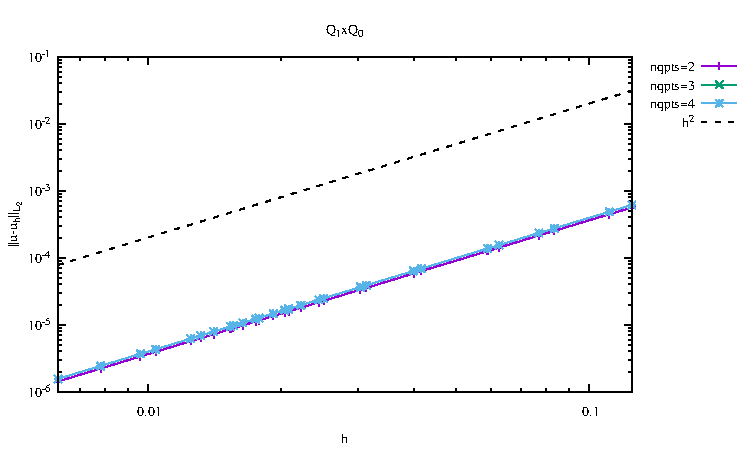
\includegraphics[width=7cm]{python_codes/fieldstone_120/results/Q1Q0-velocity-h.pdf}
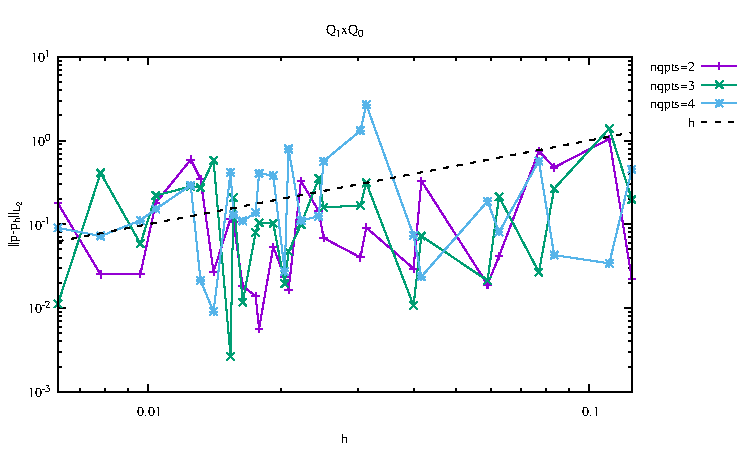
\includegraphics[width=7cm]{python_codes/fieldstone_120/results/Q1Q0-pressure-h.pdf}\\
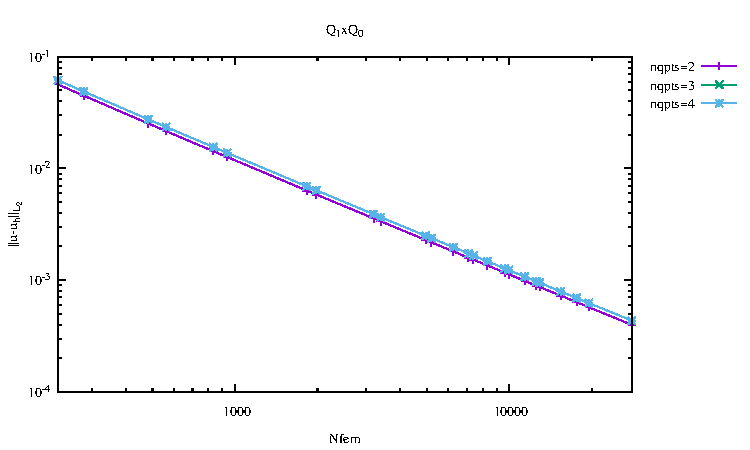
\includegraphics[width=7cm]{python_codes/fieldstone_120/results/Q1Q0-velocity-Nfem.pdf}
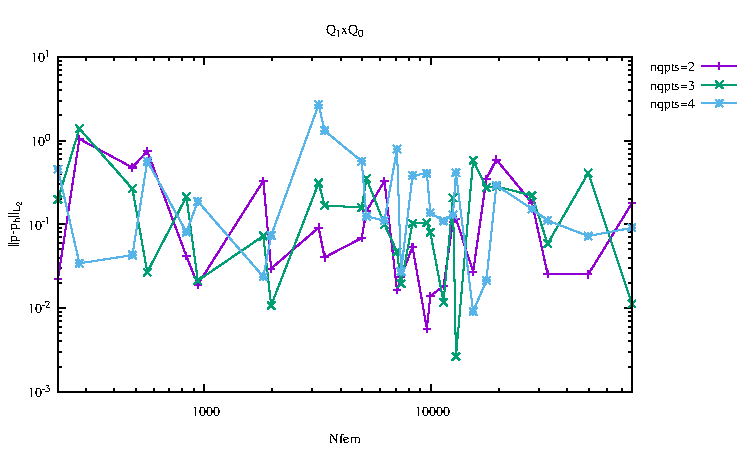
\includegraphics[width=7cm]{python_codes/fieldstone_120/results/Q1Q0-pressure-Nfem.pdf}
\end{center}


%----------------------------
\subsection*{$Q_2\times Q_1$}

\begin{center}
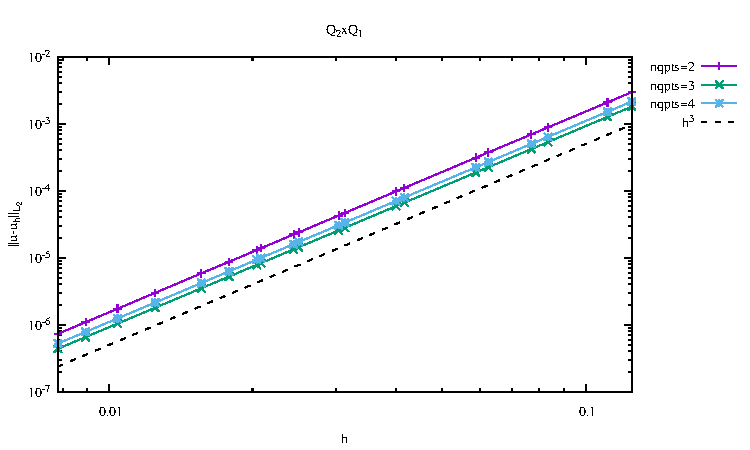
\includegraphics[width=7cm]{python_codes/fieldstone_120/results/Q2Q1-velocity-h.pdf}
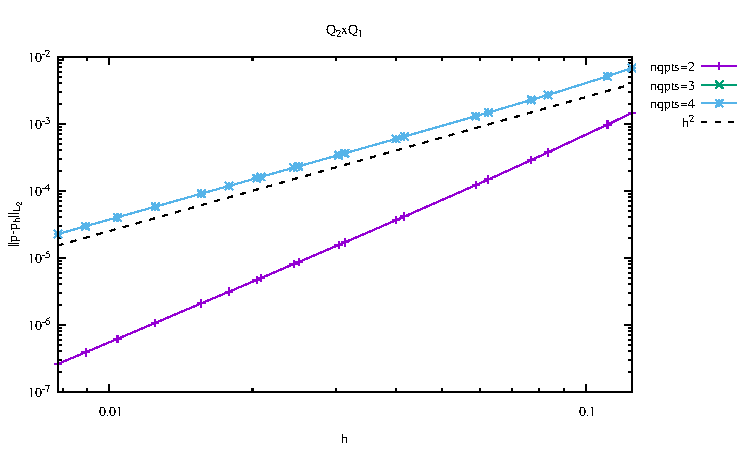
\includegraphics[width=7cm]{python_codes/fieldstone_120/results/Q2Q1-pressure-h.pdf}\\
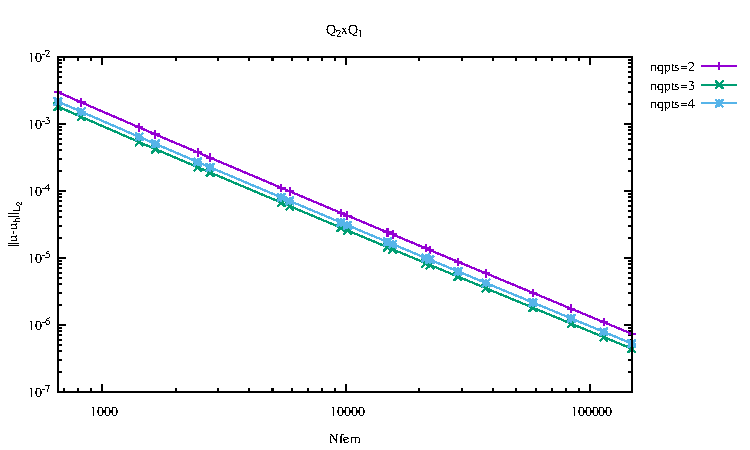
\includegraphics[width=7cm]{python_codes/fieldstone_120/results/Q2Q1-velocity-Nfem.pdf}
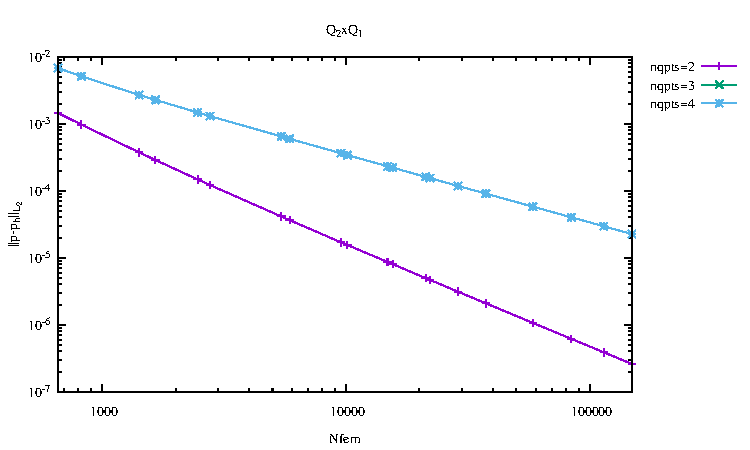
\includegraphics[width=7cm]{python_codes/fieldstone_120/results/Q2Q1-pressure-Nfem.pdf}
\end{center}

%----------------------------
\subsection*{$Q_3\times Q_2$}

\begin{center}
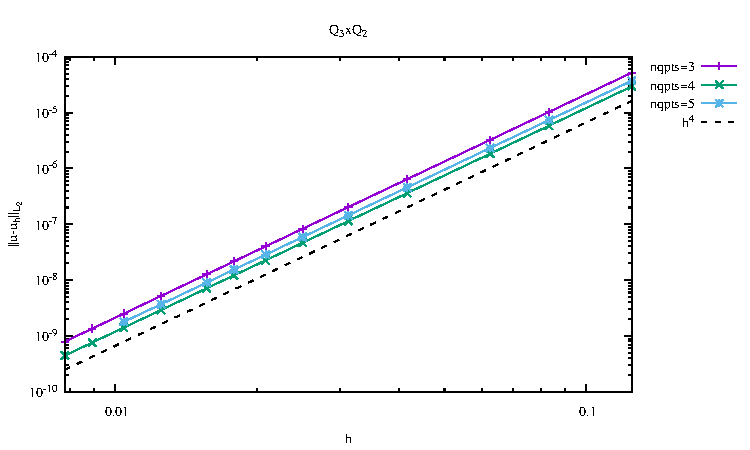
\includegraphics[width=7cm]{python_codes/fieldstone_120/results/Q3Q2-velocity-h.pdf}
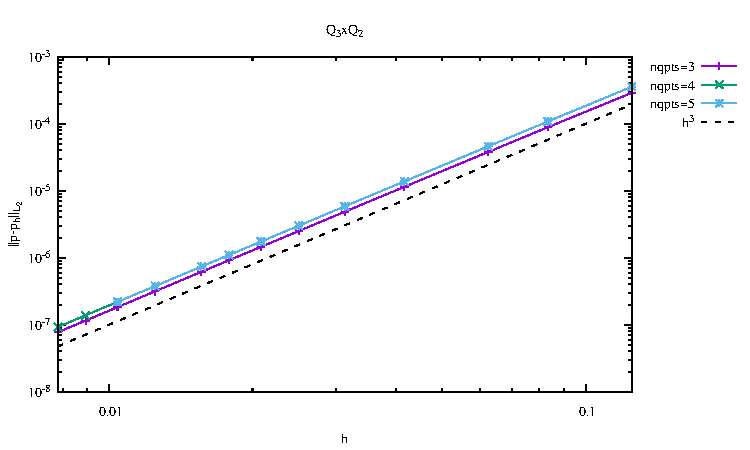
\includegraphics[width=7cm]{python_codes/fieldstone_120/results/Q3Q2-pressure-h.pdf}\\
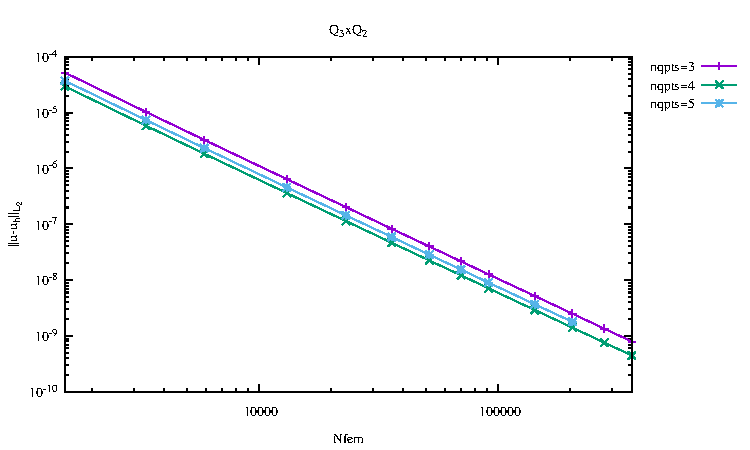
\includegraphics[width=7cm]{python_codes/fieldstone_120/results/Q3Q2-velocity-Nfem.pdf}
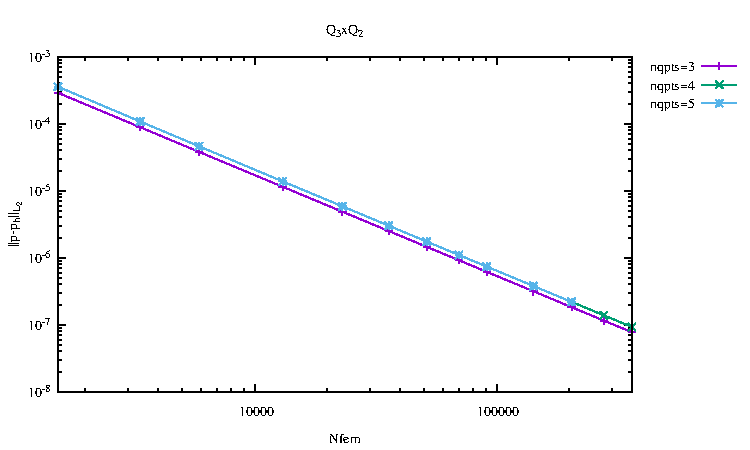
\includegraphics[width=7cm]{python_codes/fieldstone_120/results/Q3Q2-pressure-Nfem.pdf}
\end{center}

%----------------------------
\subsection*{$Q_1^+\times Q_1$}

\begin{center}
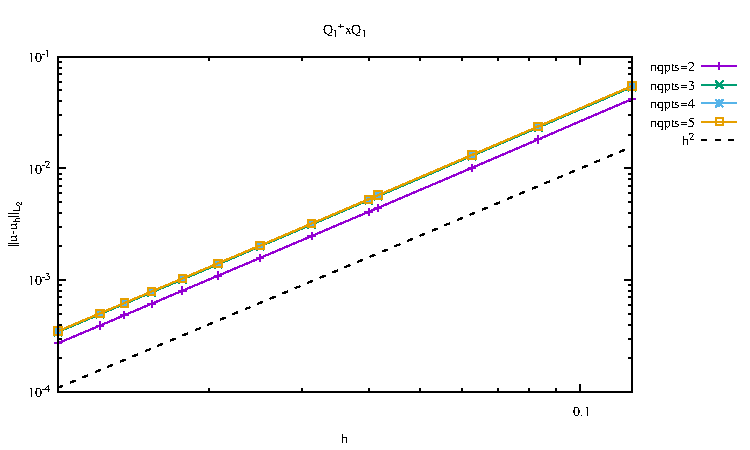
\includegraphics[width=7cm]{python_codes/fieldstone_120/results/Q1+Q1-velocity-h.pdf}
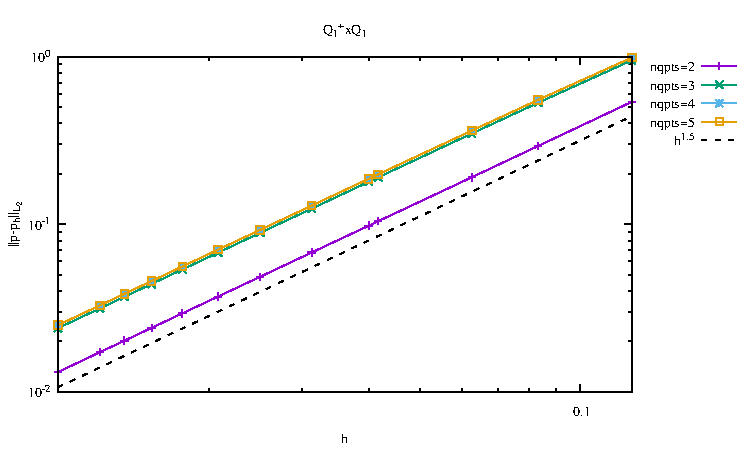
\includegraphics[width=7cm]{python_codes/fieldstone_120/results/Q1+Q1-pressure-h.pdf}
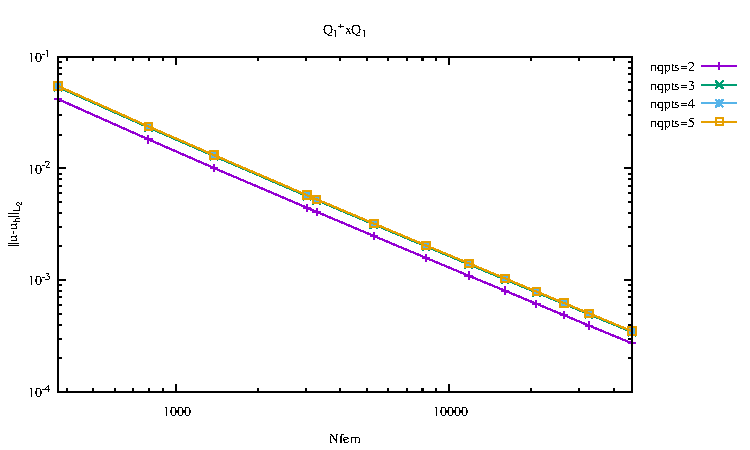
\includegraphics[width=7cm]{python_codes/fieldstone_120/results/Q1+Q1-velocity-Nfem.pdf}
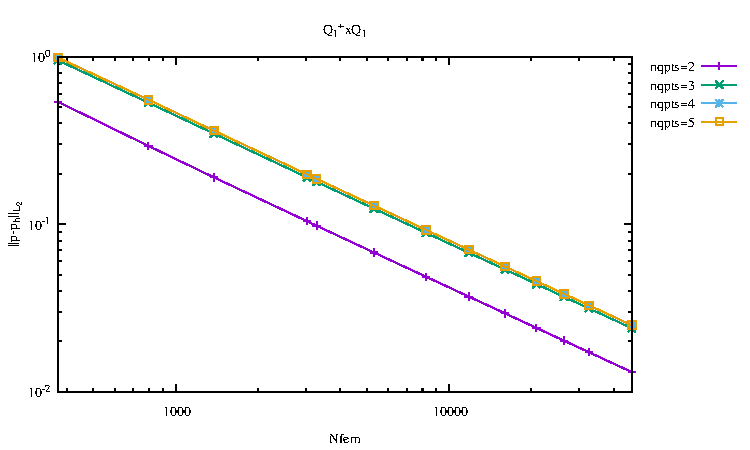
\includegraphics[width=7cm]{python_codes/fieldstone_120/results/Q1+Q1-pressure-Nfem.pdf}
\end{center}

%----------------------------
\subsection*{$P_1^+\times P_1$}
\begin{center}
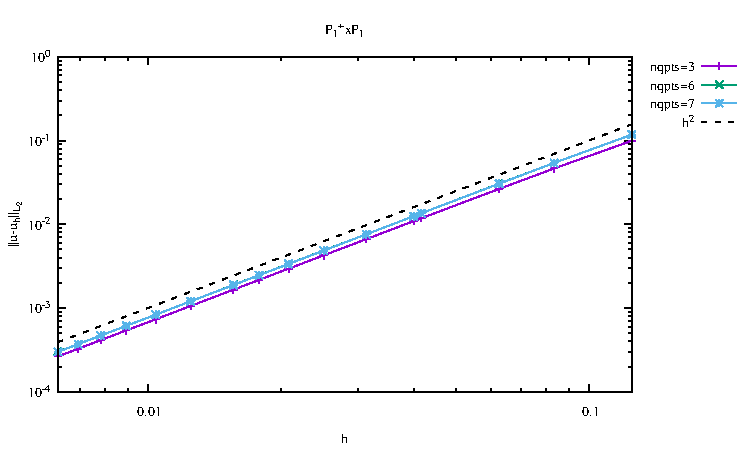
\includegraphics[width=7cm]{python_codes/fieldstone_120/results/P1+P1-velocity-h.pdf}
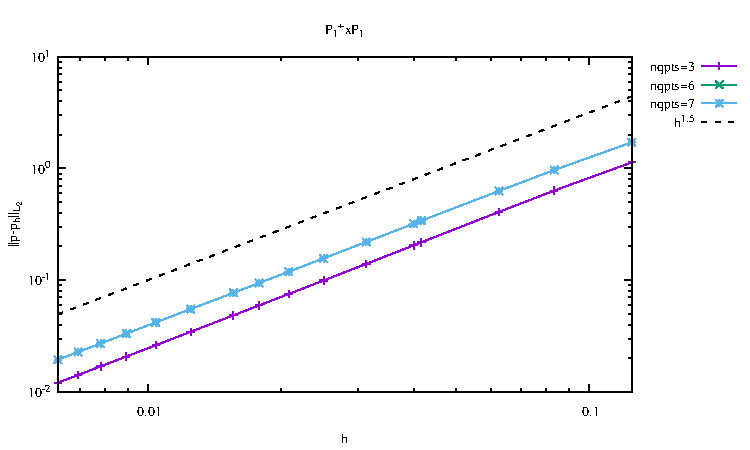
\includegraphics[width=7cm]{python_codes/fieldstone_120/results/P1+P1-pressure-h.pdf}
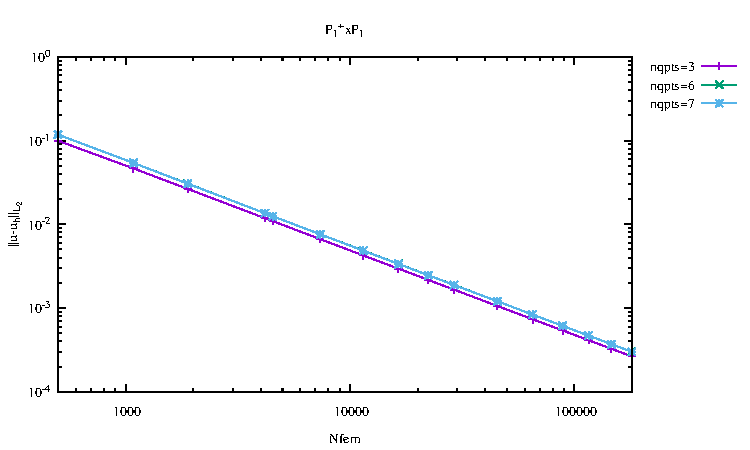
\includegraphics[width=7cm]{python_codes/fieldstone_120/results/P1+P1-velocity-Nfem.pdf}
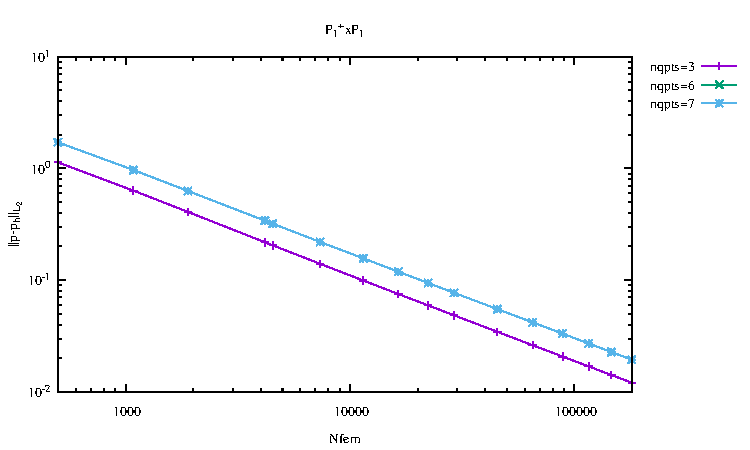
\includegraphics[width=7cm]{python_codes/fieldstone_120/results/P1+P1-pressure-Nfem.pdf}
\end{center}

%----------------------------
\subsection*{$P_2\times P_1$}
\begin{center}
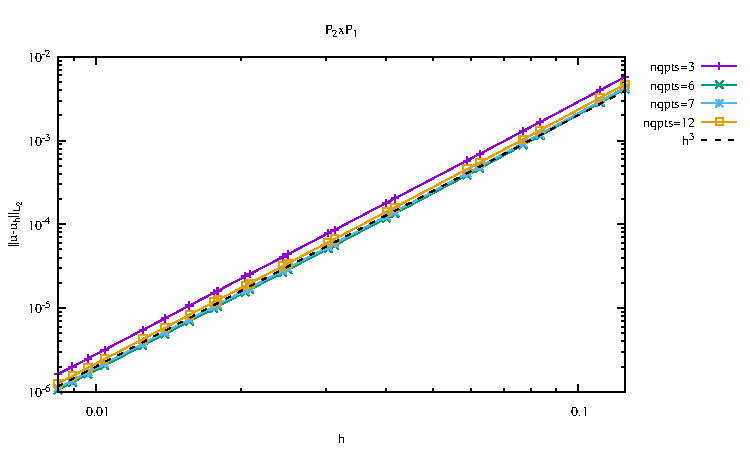
\includegraphics[width=7cm]{python_codes/fieldstone_120/results/P2P1-velocity-h.pdf}
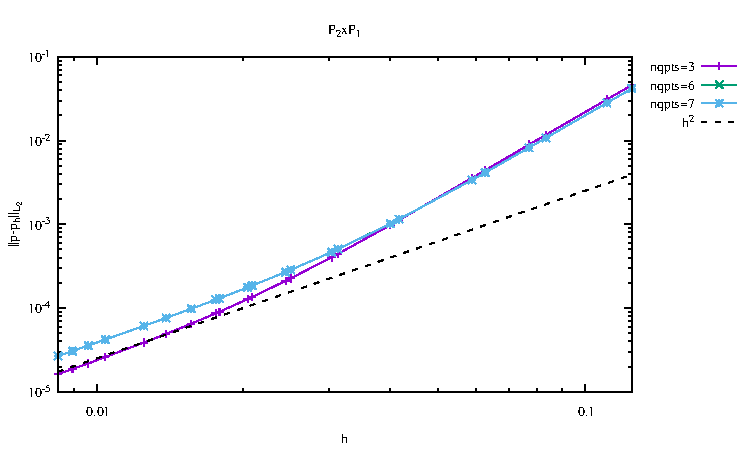
\includegraphics[width=7cm]{python_codes/fieldstone_120/results/P2P1-pressure-h.pdf}
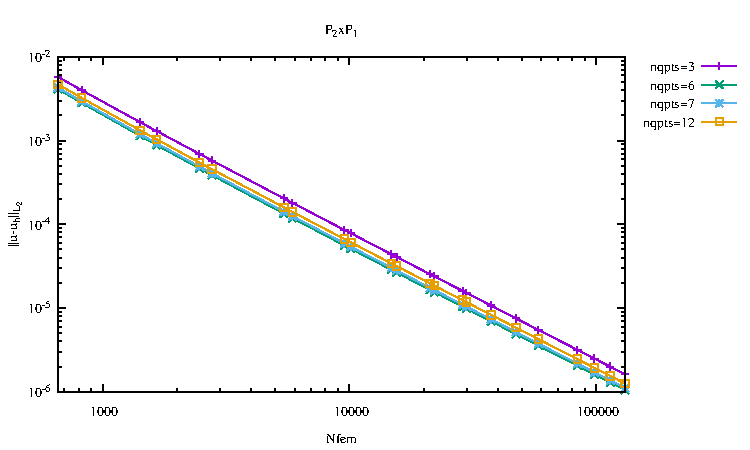
\includegraphics[width=7cm]{python_codes/fieldstone_120/results/P2P1-velocity-Nfem.pdf}
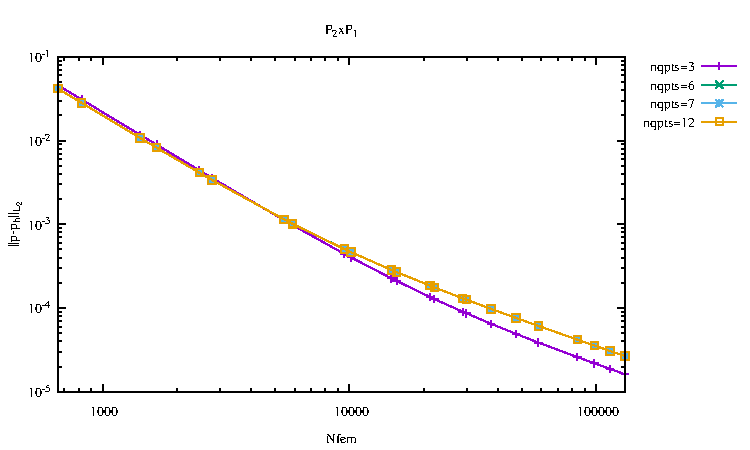
\includegraphics[width=7cm]{python_codes/fieldstone_120/results/P2P1-pressure-Nfem.pdf}
\end{center}

%----------------------------
\subsection*{$P_2^+\times P_{-1}$}
\begin{center}
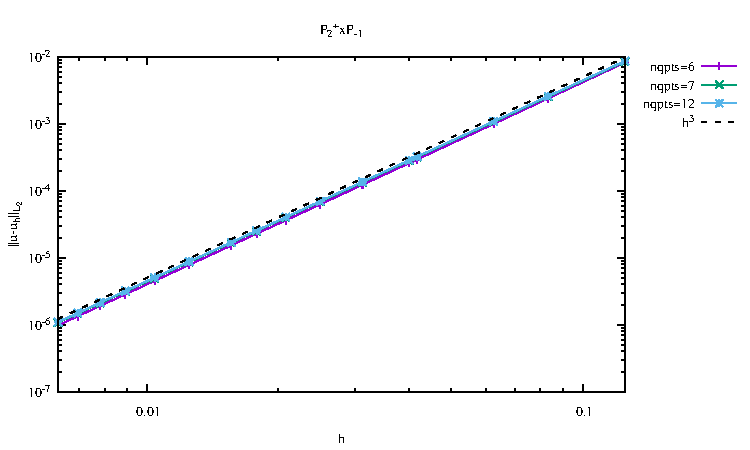
\includegraphics[width=7cm]{python_codes/fieldstone_120/results/P2+P-1-velocity-h.pdf}
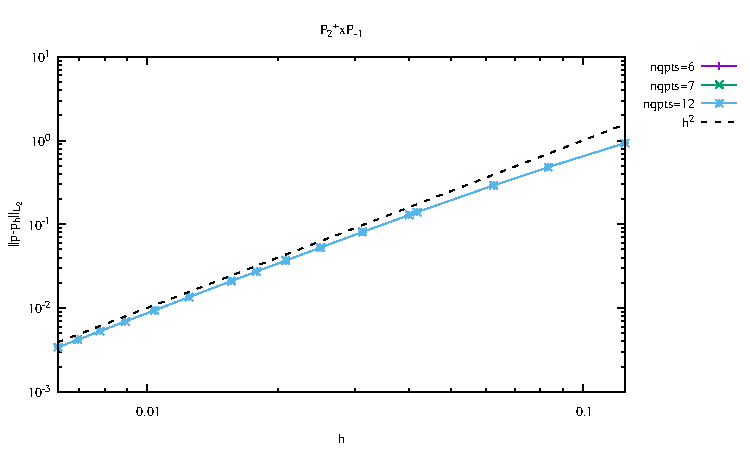
\includegraphics[width=7cm]{python_codes/fieldstone_120/results/P2+P-1-pressure-h.pdf}
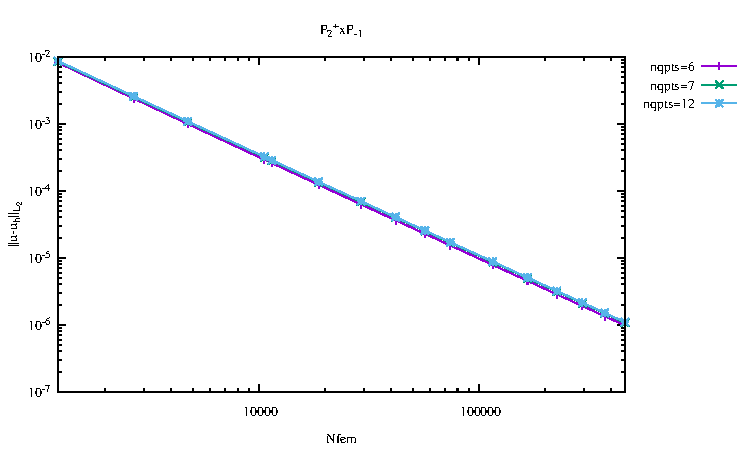
\includegraphics[width=7cm]{python_codes/fieldstone_120/results/P2+P-1-velocity-Nfem.pdf}
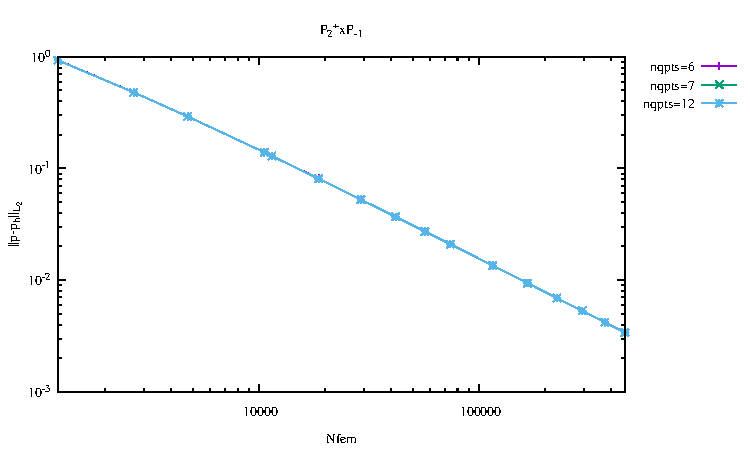
\includegraphics[width=7cm]{python_codes/fieldstone_120/results/P2+P-1-pressure-Nfem.pdf}
\end{center}

%----------------------------
\subsection*{$P_3\times P_2$}
\begin{center}
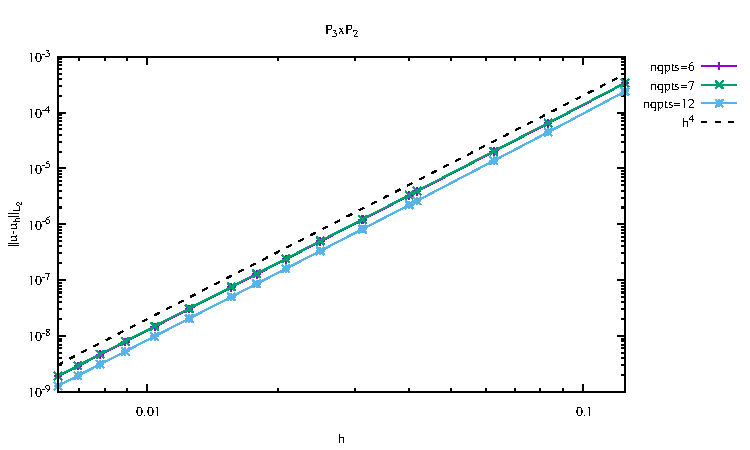
\includegraphics[width=7cm]{python_codes/fieldstone_120/results/P3P2-velocity-h.pdf}
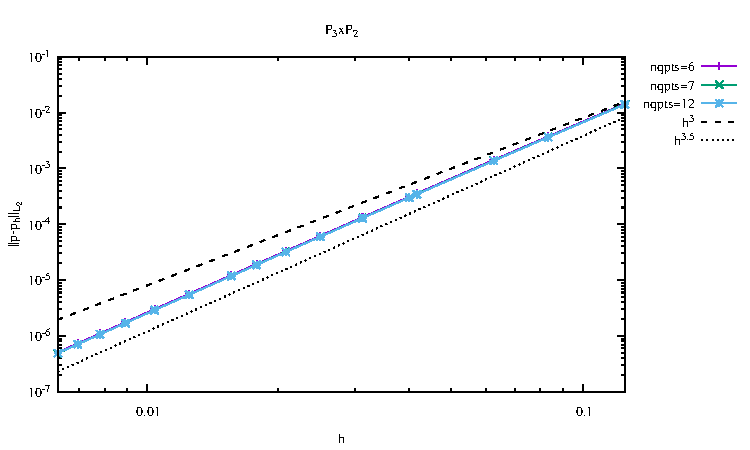
\includegraphics[width=7cm]{python_codes/fieldstone_120/results/P3P2-pressure-h.pdf}
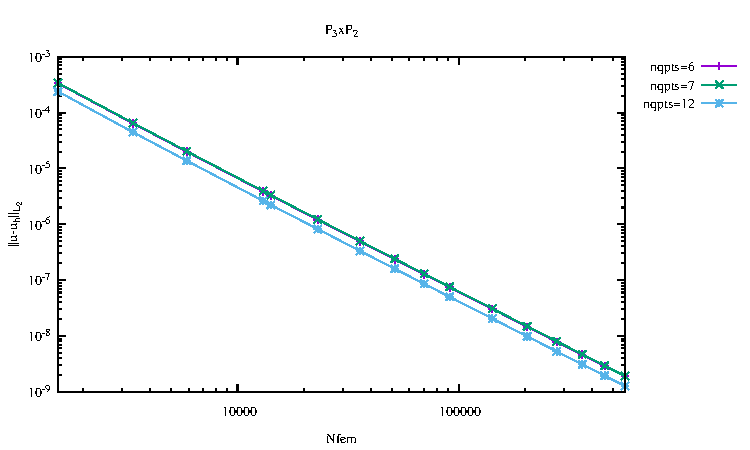
\includegraphics[width=7cm]{python_codes/fieldstone_120/results/P3P2-velocity-Nfem.pdf}
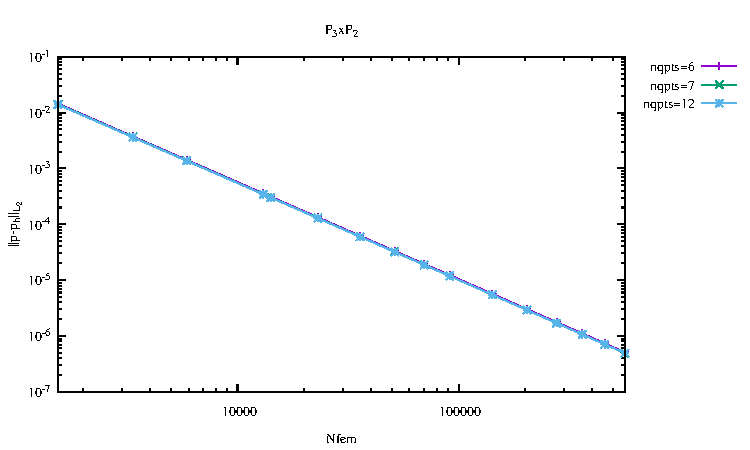
\includegraphics[width=7cm]{python_codes/fieldstone_120/results/P3P2-pressure-Nfem.pdf}
\end{center}

%----------------------------
\subsection*{$Q_1\times Q_0$-RT1}
\begin{center}
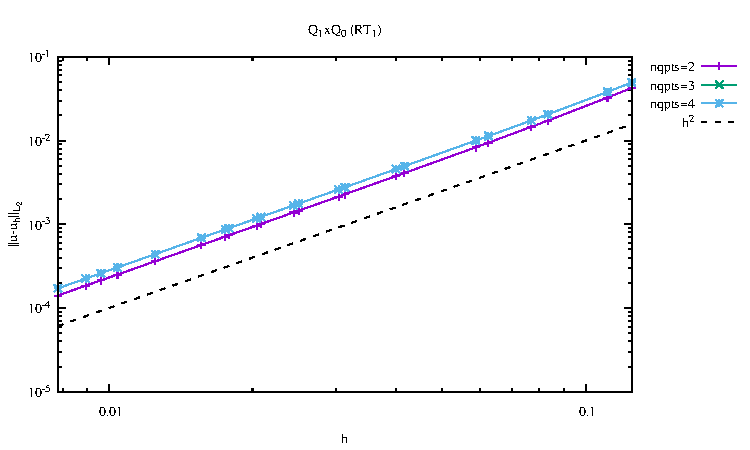
\includegraphics[width=7cm]{python_codes/fieldstone_120/results/RT1Q0-velocity-h.pdf}
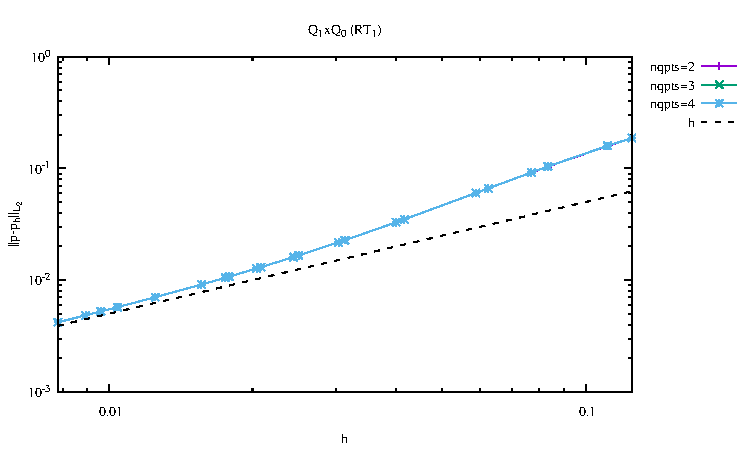
\includegraphics[width=7cm]{python_codes/fieldstone_120/results/RT1Q0-pressure-h.pdf}
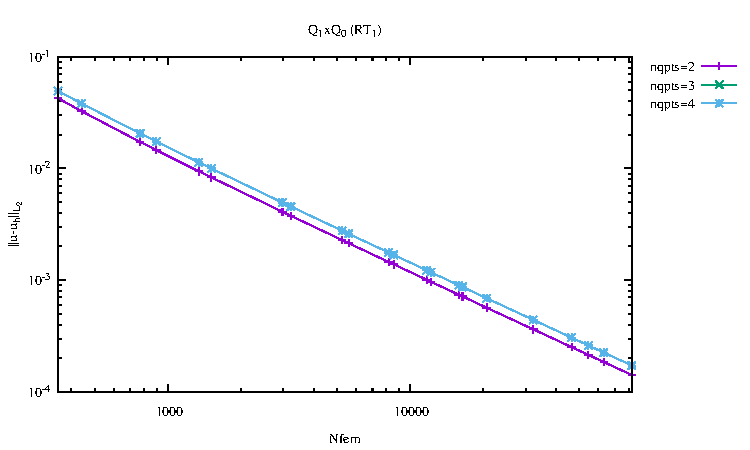
\includegraphics[width=7cm]{python_codes/fieldstone_120/results/RT1Q0-velocity-Nfem.pdf}
\includegraphics[width=7cm]{python_codes/fieldstone_120/results/RT1Q0-pressure-Nfem.pdf}
\end{center}

%----------------------------
\subsection*{$Q_1\times Q_0$-RT2}
\begin{center}
\includegraphics[width=7cm]{python_codes/fieldstone_120/results/RT2Q0-velocity-h.pdf}
\includegraphics[width=7cm]{python_codes/fieldstone_120/results/RT2Q0-pressure-h.pdf}
\includegraphics[width=7cm]{python_codes/fieldstone_120/results/RT2Q0-velocity-Nfem.pdf}
\includegraphics[width=7cm]{python_codes/fieldstone_120/results/RT2Q0-pressure-Nfem.pdf}
\end{center}

%----------------------------
\subsection*{$Q_1\times Q_0$-DSSY1}
\begin{center}
\includegraphics[width=7cm]{python_codes/fieldstone_120/results/DSSY1Q0-velocity-h.pdf}
\includegraphics[width=7cm]{python_codes/fieldstone_120/results/DSSY1Q0-pressure-h.pdf}
\includegraphics[width=7cm]{python_codes/fieldstone_120/results/DSSY1Q0-velocity-Nfem.pdf}
\includegraphics[width=7cm]{python_codes/fieldstone_120/results/DSSY1Q0-pressure-Nfem.pdf}
\end{center}

%----------------------------
\subsection*{$Q_1\times Q_0$-DSSY2}
\begin{center}
\includegraphics[width=7cm]{python_codes/fieldstone_120/results/DSSY2Q0-velocity-h.pdf}
\includegraphics[width=7cm]{python_codes/fieldstone_120/results/DSSY2Q0-pressure-h.pdf}
\includegraphics[width=7cm]{python_codes/fieldstone_120/results/DSSY2Q0-velocity-Nfem.pdf}
\includegraphics[width=7cm]{python_codes/fieldstone_120/results/DSSY2Q0-pressure-Nfem.pdf}
\end{center}



\newpage
%------------------------------
\subsection*{Altogether}


\begin{center}
\includegraphics[width=8.5cm]{python_codes/fieldstone_120/results/errors-velocity-all}
\includegraphics[width=8.5cm]{python_codes/fieldstone_120/results/errors-pressure-all}\\
\includegraphics[width=10cm]{python_codes/fieldstone_120/results/vrms-Nfem}
\end{center}


